\scanpage{13}\mspage{12}
\deleted{\unsure{pre|pr}}include either $\leq$, or $\triangleleft$.

\deleted{b) $\leq$ and $\ll$ \unsure{determine} $\preccurlyeq$, for}
\[
\deleted{G\preccurlyeq F\Longleftrightarrow G\ll F}
\]

b) Each of the relations $\leq$, $\ll$ determines the relation $\parallel$. Indeed
\[
\left\{\begin{aligned}
\text{a)}\quad F\parallel G &\ \deleted{\unsure{\Longleftrightarrow|\Longrightarrow}}\unsure{\Longrightarrow|\Longleftrightarrow}
 \{F,G\}\ \text{bounded above for }\leq,\ \text{and }\mathop{\mathrm{Inf}}\limits_{\leq}(F,G)=\varnothing_F\\
\text{b)}\quad F\parallel G &\ \Longleftrightarrow
 \deleted{\unsure{\mathrm{Inf}|\mathrm{S}}}\mathop{\mathrm{Sup}}\limits_{\ll}(F,G)\ \text{exists, and }\mathop{\mathrm{Inf}}\limits_{\ll} F,G=\varnothing_F
\end{aligned}\right.
\tag*{(1.24)}
\]
\margin{Check $\longrightarrow$}
(\uline{NB} $\varnothing_{\unsure{\mathcal{F}|\mathfrak{F}}}$ is the least \unsure{element|element} of $\mathcal{F}$ both for $\leq$, and for $\ll$)

c) The relation $\ll$ determines $\preccurlyeq$, by
\margin{$\times$}
\[
\begin{aligned}
F\preccurlyeq G &\Longleftrightarrow F\ll G,\ \text{and }\forall H\underset{\deleted{\leq}}{\in}\mathcal{F}\deleted{\unsure{H|K}}\ \text{we have}\\
&\hspace{2em}(H\parallel F\Longleftrightarrow H\parallel G)
\end{aligned}
\tag*{(1.25)}
\]
and we apply b).

d) The relation $\ll$ determines $\mathcal{L}\subset\mathcal{F}$ as the set of minimal elements of $\mathcal{F}\setminus\{\varnothing_{\mathcal{F}}\}$:
\[
\mathcal{L}=\bigl\{\substack{X\in\mathcal{F}\\ X\neq\varnothing_{\mathcal{F}}}\mid
 Y\in\mathcal{F},\ Y\ll X,\ Y\neq\varnothing_{\unsure{\mathcal{F}|F|f}}\ \Rightarrow Y=X\bigr\} \tag*{(1.26)}
\]
(a \unsure{locus|link} is a nonempty figure whose only nonempty refinement is it-$\overline{\mathrm{self}}$).

\figure{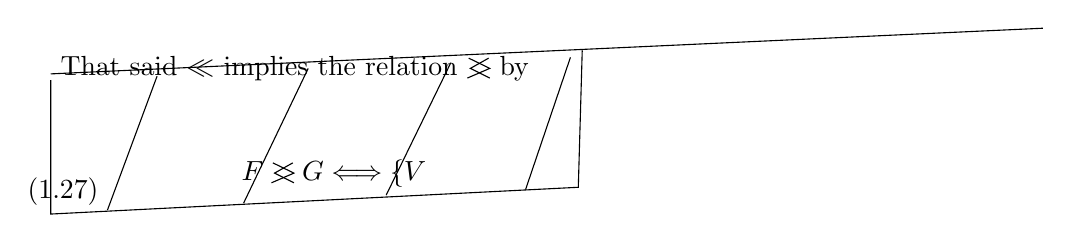
\begin{tikzpicture}[x=1cm,y=1cm]
\node[anchor=west] at (0,1.55) {\deleted{That said $\ll$ implies the relation $\mathrel{\tikz[baseline=0pt,x=1em,y=1em]{\draw (-.38,.62)--(.38,.25)--(-.43,-.10); \draw (.34,.62)--(-.32,.25)--(.38,-.10);}}$ by}};
\node[anchor=west,inner sep=0pt] at (-.3,-.02) {$\deleted{(1.27)}$};
\node[anchor=west] at (2.3,.22) {$\deleted{F \mathrel{\tikz[baseline=0pt,x=1em,y=1em]{\draw (-.38,.62)--(.38,.25)--(-.43,-.10); \draw (.34,.62)--(-.32,.25)--(.38,-.10);}} G\Longleftrightarrow\{V}$};
\draw (0,1.48)--(12.6,2.06);
\draw (0,1.40)--(0,-.30)--(6.7,.04)--(6.75,1.78);
\draw (.72,-.25)--(1.35,1.45);
\draw (2.45,-.16)--(3.27,1.55);
\draw (4.26,-.06)--(5.08,1.62);
\draw (6.03,.01)--(6.60,1.69);
\end{tikzpicture}}
I do not see that $\ll$ ($+\ \preccurlyeq$, it's all the same) determines $\leq$, nor even $\mathrel{\tikz[baseline=0pt,x=1em,y=1em]{\draw (-.38,.62)--(.38,.25)--(-.43,-.10); \draw (.34,.62)--(-.32,.25)--(.38,-.10);}}$. But

\textcircled{\unsure{e|$\ominus$}}\quad $\ll$ and $\mathrel{\tikz[baseline=0pt,x=1em,y=1em]{\draw (-.38,.62)--(.38,.25)--(-.43,-.10); \draw (.34,.62)--(-.32,.25)--(.38,-.10);}}$ determine $\leq$ by
\margin{$\times$}
\[
G\leq F\quad\unsure{\Longleftarrow|\Longleftrightarrow}\quad (G\ll F\ \text{and}\ G \mathrel{\tikz[baseline=0pt,x=1em,y=1em]{\draw (-.38,.62)--(.38,.25)--(-.43,-.10); \draw (.34,.62)--(-.32,.25)--(.38,-.10);}} F) \tag*{(1.27)}
\]

So finally,
